\documentclass{kththesis}


%Taken from ID1354
\usepackage[utf8]{inputenc}
\usepackage[english]{babel}
\usepackage{graphicx}
\graphicspath{./images/}
\usepackage{lastpage}
\usepackage{pgf}
\usepackage{wrapfig}
\usepackage{fancyvrb}
\usepackage{fancyhdr}
\pagestyle{fancy}
\usepackage{dingbat}

\usepackage[autostyle]{csquotes}
\usepackage[
    backend=biber,
    style=ieee,
    sortlocale=de_DE,
    natbib=true,
    url=true,
    doi=true,
    eprint=false
]{biblatex}
\addbibresource{references.bib}

\usepackage[]{hyperref}
\hypersetup{
    colorlinks=true,
}

% List of abbreviations
\usepackage[refpage]{nomencl}
\makenomenclature

\title{This is the English title}
\alttitle{Detta är den svenska översättningen av titeln}
\author{Jacob Kimblad}
\email{jacobki@kth.se}
\supervisor{Matthias Becker}
\examiner{Zhonghai Lu}
\programme{Master's Programme in Embedded Systems}
\school{School of Electrical Engineering and Computer Science}
\date{\today}


\begin{document}

% Frontmatter includes the title page, abstracts and table-of-contents
\frontmatter

\titlepage

\begin{abstract} 

    English abstract goes here.

\end{abstract}


\begin{otherlanguage}{swedish} 
    
    \begin{abstract}

    \end{abstract} 

\end{otherlanguage}


\printnomenclature


\tableofcontents


% Mainmatter is where the actual contents of the thesis goes
\mainmatter


\chapter{Introduction} 

Embedded systems in the automotive sector are required to go through a lot of analysis and testing
before being deemed safe for use in traffic. With the rise of autonomous vehicles these systems are
becoming more complex as an effect of more computing needed being done.  This has also put
requirements on the hardware to become faster and faster, thus the industry is turning to the use of
multi-core and many-core platforms. These type of platforms present more unpredictability than
single-core platforms which requires new methods of analysis and deterministic execution of these
systems. 


\section{Background} 

Timing analysis is an important part of real-time systems. However, multi-core platforms often
implement complicated memory hierarchies that make timing analysis a lot harder. One way to tackle
this is to schedule the access to shared memory in cooperation with computational tasks. This can
improve analysis and is employed by industrial domains already where the execution of tasks can be
divided up into three distinct parts, read-execute-write.


\section{Problem}

An analysis method for resource contention in multi-core real-time systems have been proposed in
paper [1]. This analysis method is however not 1 Template for project proposal 2018-12-12 customised
for the read-execute-write execution model that is adapted both within the avionics domain and
automotive domain.


\section{Purpose}

The purpose is to expand existing analysis methods by adding to the source code and/or produce a
model of the read-execute-write task model that is available as input for these formal analysis
methods.


\section{Goal}



\subsection{Benefits, Ethics and Sustainability}

\section{Methodology / Methods}

\section{Delimitations}

\section{Outline}


%We use the \emph{biblatex} package to handle our references.  We therefore use the command
%\texttt{parencite} to get a reference in parenthesis, like this \parencite{heisenberg2015}.  It is
%also possible to include the author as part of the sentence using \texttt{textcite}, like talking
%about the work of \textcite{einstein2016}.

\chapter{<Theoretic Background> Use a self-explaining title}



\section{The Task Model}

A task is a unit of work that is to be completed repetitively by executing on a processor over and
over again where each iteration of execution is defined as a unique job. In embedded systems a job
is usually completed in some set amount of time, this is known as its execution time which is the
same for all jobs in a task. Once a job is finished executing the task will usually wait for some
amount of time before its next job needs to execute, this is known as the tasks period. For each
multiple of the period a new job is released, this time is known as the release time and is unique
to each job within a single task.  The job is also required to be finished before a set amount of
time from its release time, this is known as the jobs absolute deadline.  For an
OS\nomenclature{OS}{Operating System} to decide in what order the jobs should be executed they each
are also assigned a priority by a scheduler, this is discussed in section \ref{sec:scheduling}.

Using the above definitions we can ascribe properties to tasks telling us what state they are in
during a set time. After a job is released and is currently being executed the task which it belongs
to can be described as currently running. Once the job is finished and the next job from the same
task is yet to be released the task can be described as waiting before once again a job belonging to
the tasks starts executing and the task is running. Once a job is running it may require access to
some resource that is not ready to be accessed yet. Instead of the job taking up time on the
processor we can pause it and let some other job execute instead. We would then say that the task is
waiting. Once the resource is available again the task can be said to be ready before its job is
allowed to continue execution.


\begin{figure}

    \centering

    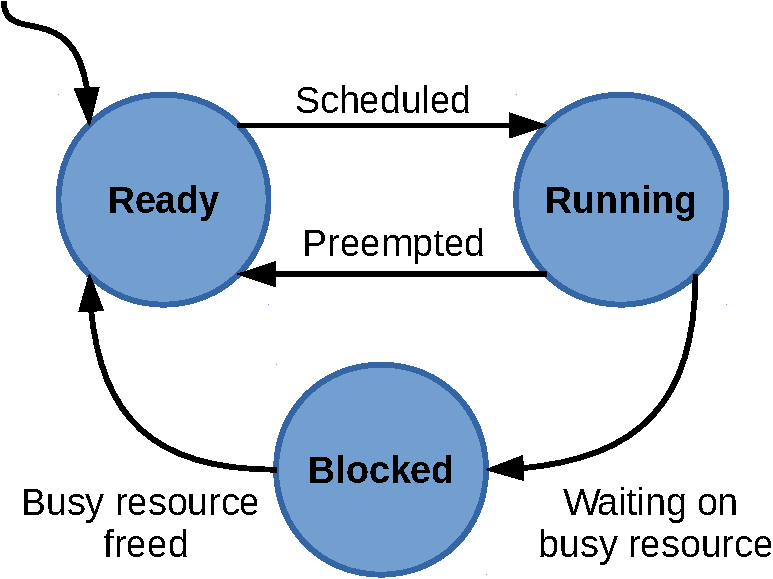
\includegraphics[scale=1\linewidth, bb=0 0 0 0]{images/ready-running-blocked-model.pdf}

    \caption{The physical setup of the hardware running the experiments.}

    \label{fig:experiment_setup}

\end{figure}

% TODO: talk about aperiodic and sporadic tasks as well? 

\section{Scheduling} \label{sec:scheduling}

Although computer give away the illusion of being able to deal with very many things simultaneously
this is actually not the case. Computers are limited to how much parallel computing they are able to
do by the hardware, specifically the amount of cores within the CPU\nomenclature{CPU}{Central
Processing Unit}. A computer with, for example, four cores is able to do at most four things in
parallel at any one time. For a computer to deal with more than four calculations require it to
switch ongoing calculations in and out of a core. These calculations are often referred to as tasks,
where tasks often produce some type of results that can be used either by the user of the computer
or another task on the system. For systems with more than one processor or processor core in it the
result may even be used by another computer. For an OS\nomenclature{OS}{Operating System} to give
the illusion being able to execute many programs in parallel it needs to schedule the tasks
according to some order. By scheduling tasks and switching them in and out of the processor very
quickly the OS is able to perform many different calculations seemingly at the same time.

The order in which tasks are scheduled is determined by a scheduler,

\section{The AER Execution Model}

The AER \nomenclature{AER}{Acquisition Execution Restitution} execution model was first proposed in
\parencite{durrieu_predictable_2014} to improve performance and predictability while using COTS
\nomenclature{COTS}{Commercial-off-the-Shelf} multi-core processors with distributed memory in the
avionics industry. Since the bottleneck for these types of systems often is the access to shared
memory AER focuses on making it more deterministic and easier to analyse. This is done by dividing
up the tasks that run within an OS\nomenclature{OS}{Operating System} into three distinct parts.

%TODO Do we first explain what a task is, that it runs on a single core within a multi-processor and
%that for this industry it often is non-greedy when it is non-preemptive. Do we go into detail of
%the task model (running, ready and executing), this is probably good to cover in the global
%scheduling part.

The paper \parencite{maia_closer_2016} takes a closer look i


\chapter{<Engineering-related content, Methodologies and Methods> Use a self-explaining title}

\nomenclature{AER}{Acquisition Execution Restitution}

\chapter{<The work> Use a self-explaining title}


\chapter{<Result> Use a self-explaining title}


\chapter{<Conclusions> Use a self-explaining title}


\printbibliography[heading=bibintoc] % Print the bibliography (and make it appear in the table of
    %contents)


\appendix

\chapter{Unnecessary Appended Material}

\end{document}
